\chapter{Aplikacja do obliczeń numerycznych}
\label{cha:aplikacja}

W tym rozdziale przedstawione są wszystkie niezbędne informacje potrzebne do korzystana ze zbudowanej na potrzeby projektu aplikacji. Aplikacja napisana jest w skryptowym języku Python. W projekcie skorzystano z gotowej paczki bibliotek Anaconda, zawierającej też potrzebny do uruchamiani programów interpreter języka. IDE wykorzystanym do tworzenia projektu jest PyCharm. Anaconda jak i wersja Community programu PyCharm są całkowicie darmowe dla zastosowań niekomercyjnych. W dalszej części rozdziału przedstawiony jest sposób instalacji i konfiguracji środowiska dla systemu Windows 8 64-bit.

Aplikacja składa się  z dwóch głównych części. Pierwsza obejmuje obliczanie modelu MES oraz wyznaczanie krzywch dyspersji i wzbudzalności na podstawie obliczonego modelu, a druga pozwla symulować propagację fali oraz metody kompensacji dyspersji. Każdy plik z roszerzeniem .py zawierający kod w Pythonie nazywa się modułem. Każda ze wspomnianych części aplikacji składa się z kilku modułów. Oprócz tego jest kilka modułów z funkcjami pomocniczymi wykorzystywanymi w głównych częściach programu. Wszystkie moduły zostaną omówione w dalszej części rozdziału.

\section{Instalacja i konfiguracja środowiska}
\label{sec:instalacja}

\subsection{Anaconda}
\label{sec:anaconda}

Instalację rozpoczynamy od interpretera Python. Pliki instalacyjne pobrać można z oficjalnej strony Python \hyperref[python]{''https://www.python.org/ ''}. Na stronie powinniśmy znaleźć pliki instalacyjne kolejnych wersji dla różnych systemów operacyjnych. Pobieramy plik odpowiedni dla naszego systemu. W omawianym przypadku będzie to win-64. Pliki instalacyjne zawarte są na płycie CD dołączonej do pracy. W projekcie korzystanu z wersji Python 3.6.3.

Po zainstalowaniu Pythona należy dodać ścieżkę do zmiennych systemowych. W tym celu wymagane są uprawnienie administratora. Poniżej znajdują się instrukcja dodawania ścieżki oraz sposób sprawdzenia czy Python jest widoczny przez system.

Otwieramy ,,Panel Sterowania'' (,,Control Panel''). Wchodzimy w zakładkę ,,System i Zabezpieczenia'' (,,System and Security''), rysunek \ref{fig:anaconda1}, a następnie w ,,System'', rysunek \ref{fig:anaconda2}. Z lewej strony klikamy ,,Zaawansowane ustawienia systemu'' (,,Advanced system settings''), rysunek \ref{fig:anaconda3}, a następnie
,,Zmienne środowiskowe'' (,,Environment variables''), rysunek \ref{fig:anaconda4}. Znajdujemy zmienną ,,Ścieżka'' (,,Path''), rysunek \ref{fig:anaconda5} i otwieramy ją przez dwukrotne kliknięcie myszką. Przesuwamy do końca tekst w nowo otwartym oknie i dopisujemy na końcu średnik, ścieżkę do folderu gdzie zainstalowaliśmy Pythona, kolejny średnik i ścieżkę do folderu Scripts, który znajduje się w katalogu instalacji, rysunek \ref{fig:python6}. Przykładowe ścieżki to ;F:\textbackslash Programy\textbackslash Python;F:\textbackslash Programy\textbackslash Python\textbackslash Scripts. We wszystkich oknach które otworzyliśmy klikamy OK.

Aby sprawdzić czy całość operacji przebiegła pomyślnie należy otworzyć ,,Wiersz Poleceń'' (,,Command Prompt''), np. poprzez kliknięcie symbulu Windows na klawiaturze, wpisanie ,,cmd'' i otwarcie znalezionej aplikacji.W otwartym oknie wpisujemy komendę ,,python'', rysunek \ref{fig:python7}.  Jeśli jest ona rozpoznana to dostaniemy odpowiedź jak na rysunku \ref{fig:python8}. Jeśli komenda nie zostanie rozpoznana, należy sprawdzic poprzednie kroki oraz prawidłowość ścieżek dodanych do zmiennej ,,Path''.

\begin{figure}[h]
\centering
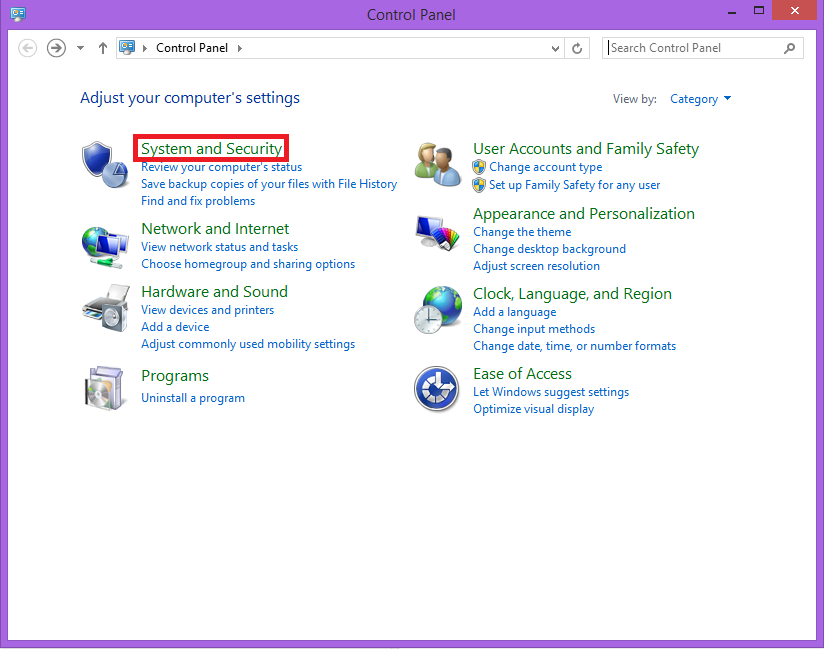
\includegraphics[width=14cm]{Zdjecia/5/anaconda1}
\caption{Widok panelu sterowania}
\label{fig:anaconda1}
\end{figure}

\begin{figure}[h]
\centering
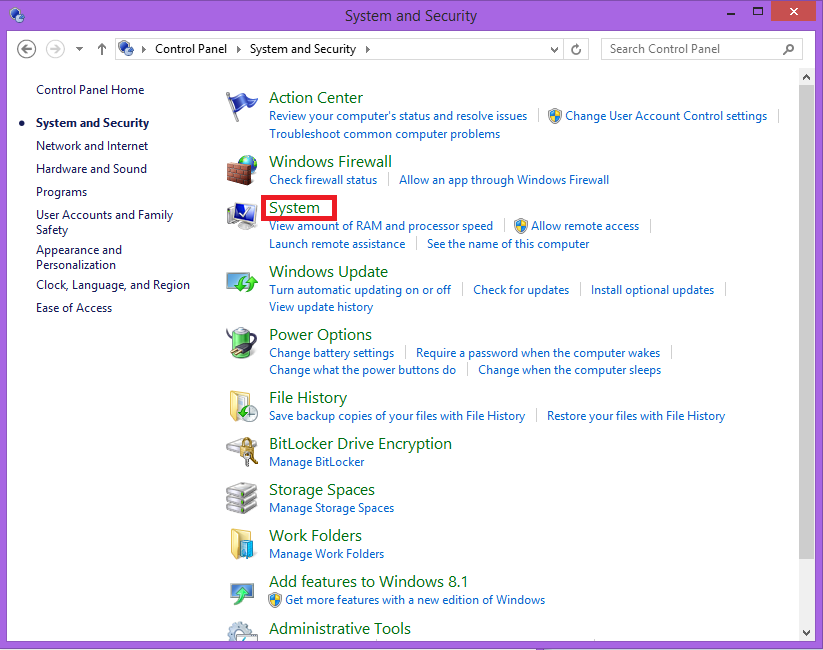
\includegraphics[width=14cm]{Zdjecia/5/anaconda2}
\caption{Zakłada System i Zabezpieczenia}
\label{fig:anaconda2}
\end{figure}

\begin{figure}[h]
\centering
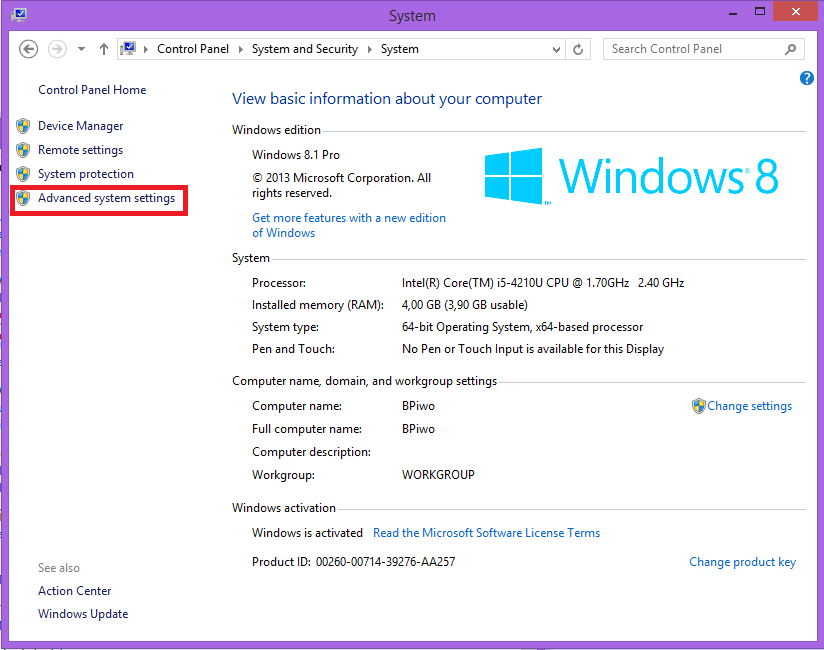
\includegraphics[width=14cm]{Zdjecia/5/anaconda3}
\caption{Zakładka System}
\label{fig:anaconda3}
\end{figure}

\begin{figure}[h]
\centering
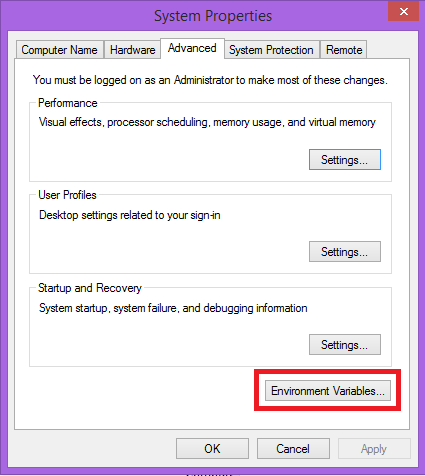
\includegraphics[width=10cm]{Zdjecia/5/anaconda4}
\caption{Okno Zaawansowane ustawienia systemu}
\label{fig:anaconda4}
\end{figure}

\begin{figure}[h]
\centering
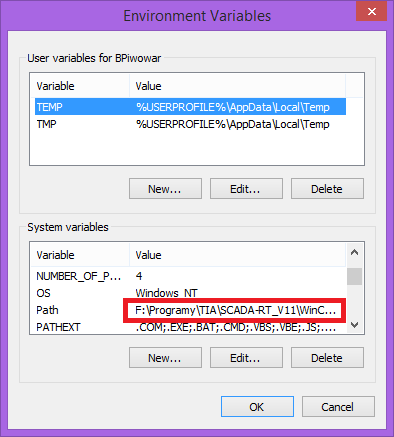
\includegraphics[width=10cm]{Zdjecia/5/anaconda5}
\caption{Okno Zmienne środowiskowe}
\label{fig:anaconda5}
\end{figure}

\begin{figure}[h]
\centering
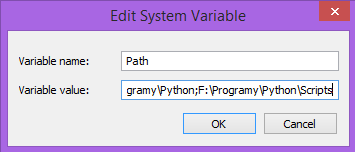
\includegraphics[width=10cm]{Zdjecia/5/python6}
\caption{Okno zmiennej Path}
\label{fig:python6}
\end{figure}


\begin{figure}[h]
\centering
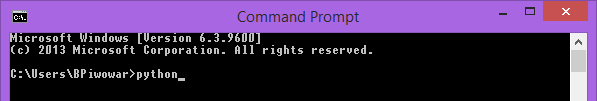
\includegraphics[width=14cm]{Zdjecia/5/python7}
\caption{Wiersz Poleceń}
\label{fig:python7}
\end{figure}

\begin{figure}[h]
\centering
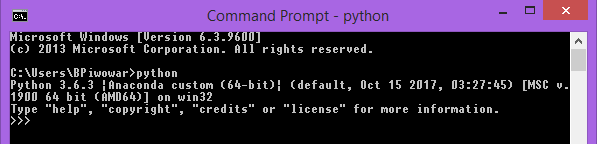
\includegraphics[width=14cm]{Zdjecia/5/python8}
\caption{Odpowiedź na komendę ,,Conda''}
\label{fig:python8}
\end{figure}

\subsection{PyCharm}
\label{sec:pycharm}

IDE wykorzystywanym w projekcie jest PyCharm. Program jest dostępny do pobrania pod linkiem https:\textbackslash \textbackslash www.jetbrains.com\textbackslash pycharm\textbackslash download\textbackslash \#section=windows. Dodatkowo plik instalacyjny jest zamieszczony na płycie CD dołączonej do pracy. Po zainstalowaniu programu, można otworzyć projekt aplikacji w standardowy sposób tj. File -> Open. W oknie, które się otworzy należy wskazać katalog projektu.

Ostatnia rzecz dotycząca konfiguracji to ustawienie aktywnego interpretera dla projektu. W tym celu należy wejść w ustawienia (,,Settings''), rysunek \ref{fig:pycharm1}. Następnie otwieramy zakładkę ,,Project'', klikamy na ,,Project interpreter'' i w pasku wyboru na górze wybieramy interpreter ze ścieżką, gdzie zainstalowaliśmy Pythona, rysunek \ref{fig:pycharm2}.

\begin{figure}[h]
\centering
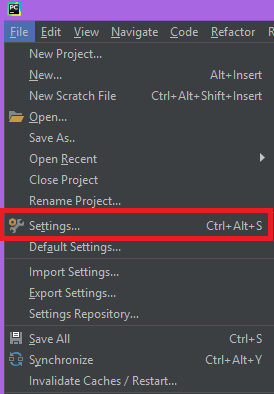
\includegraphics[width=10cm]{Zdjecia/5/pycharm3}
\caption{Okno główne projektu w programie PyCharm}
\label{fig:pycharm1}
\end{figure}

\begin{figure}[h]
\centering
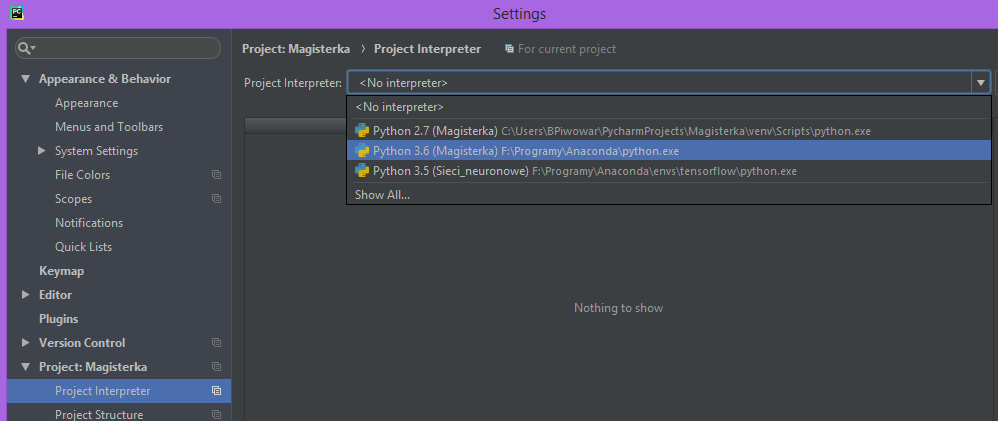
\includegraphics[width=14cm]{Zdjecia/5/pycharm4}
\caption{Wybór interpretera}
\label{fig:pycharm2}
\end{figure}












\section{Obliczenia MES i wyznaczanie krzywych dyspersji oraz wzbudzalności}
\label{cha:obliczenia_mes}

W tej sekcji przedstawione są kolejno sposoby tworzenia siatki węzłów, budowy elementów skończonych, wyznaczania lokalnych i globalnych macierzy modelu MES pręta i wyznaczani krzywych dyspersji oraz wzbudzalności. Program umożliwia tworzenie modelu MES z wykorzystanie elementów czworościennych oraz sześciennych. Krzywe dyspersji oraz wzbudzalności można wyznaczyć z obliczonego modelu, ale jest też opcja wczytania danych modelu z programu MARC.

Strukturę projektu przedstawia rysunek \ref{fig:okno_projektu}. Implementacja zagadnień związanych z obliczeniami MES oraz wyznaczaniem krzywych dyspersji z obliczonego modelu znajduje się w katalogu MES\textunderscore dir. Katalog MARC zawiera funkcje umożliwiające wczytanie danych z programu MARC i na ich podstawie wyznaczeniu krzywych dyspersji.

\begin{figure}[h]
\centering
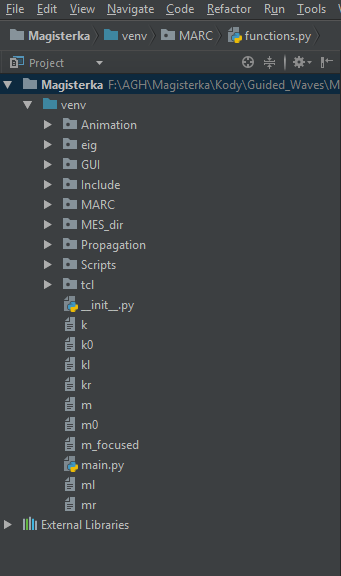
\includegraphics[width=5cm]{Zdjecia/5/okno_projektu}
\caption{Widok okna projektu}
\label{fig:okno_projektu}
\end{figure}


\subsection{Elementy czworościenne}
\label{cha:elementy czworościenne}

Zawartość katalogu MES dir przedstawia rysunek \ref{fig:okno_projektu_MES}. Obliczenia dotyczące elementów czworościennych zawarte są w modułach katalogu tetrahedralElements. Poniżej znajdują się funkcje poszczególnych modułów, wraz z opisem ich zastosowania, argumentami wejściowymi oraz wyjściowymi.

Dane zbierane w postaci macierzy są najczęściej tablicami array z biblioteki NumPy, która służy do obliczeń numreycznych. W części modułów obliczenia są prowadzone na zmiennych symbolicznych z wykorzystaniem biblitoeki SymPy. Macierze zmiennych symbolicznych są obiektami Matrix z tej biblioteki.

\begin{figure}[h]
\centering
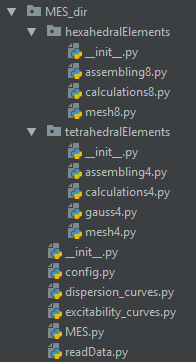
\includegraphics[width=5cm]{Zdjecia/5/okno_projektu_MES}
\caption{Widok okna projektu}
\label{fig:okno_projektu_MES}
\end{figure}

\vspace {3mm}
 \( \textbf{Moduł mesh4} \).

\vspace {3mm}
\textit{circlePlaneVerticies(x, radius, numberOfPoints)} - funkcja wykorzystywana przy tworzeniu siatki (w circleMeshFull oraz circleMeshSparse). Dodaje do siatki węzły na okręgu w jednej płaszczyźniej pręta, która znajduje się na długości x. Promień okręgu określa - radius, a ilość węzłów na okręgu - numberOfPoints.

\vspace {3mm}
\textit{circleMeshFull(radius, numberOfCircles, numberOfPoints)} - funkcja tworzy siatkę na trzech płaszczyznach przesuniętych o 1 we współrzędnej x. Siatka zbudowana jest na każdej płaszczyźnie tak samo i zawiera węzeł centralny oraz okręgi z węzłami w ilości numberOfCircles. Na każdym okręgu liczba węzłów jest większa, aby zapewnić możliwie równe odległości pomiędzy węzłami. Pierwszy okrąg zawiera liczbę węzłów numberOfPoints. Zwraca tablicę o wymiarach n x 3, gdzie n to liczba węzłów. W kolumnach są kolejne współrzędne węzłów.

\vspace {3mm}
\textit{circleMeshSparse(radius, numberOfCircles, numberOfPoints)} - jak wyżej, z tą różnicą, że każdy okrąg siatki ma tyle samo węzłów.

\vspace {3mm}
\textit{triangulation(vertices)} - funkcja tworzy elementy skończone czworościenne. Przyjmuje macierz węzłów z powyższych funkcji - vertices i zwraca tablicę e x 4, gdzie e to liczba elementów. W kolumnach zawarte są indeksy węzłów z macierzy wejściowej, które należą do danego elementu.

\vspace {3mm}
\textit{correctVolumeSign(vertices, indices)} - funkcja przyjmuje macierz współrzędnych węzłów - vertices oraz indeksy węzłów dla każdego elementu skończonego - indices. Sprawdza czy objętość elementu skończonego obliczona za pomocą wyznacznika ma dodatnią wartość. Jeśli nie, to zmienia miejscami dwa indeksy elementu w macierzy zwróconej z triangulation(vertices).

\vspace {3mm}
\textit{drawPlane(vertices)} - funkcja przyjmuje macierz współrzędnych węzłów - vertices i rysuje ich układ na płaszczyźnie. Przykładowe układu przedstawione są na rysunku \ref{fig:siatka}.

\vspace {3mm}
\textit{drawBar(vertices)} - funkcja przyjmuje macierz współrzędnych węzłów - vertices i rysuje wszystkie węzły w rzucie izometrycznym. Przykład przedstawia rysunek \ref{fig:pret}.

\vspace {3mm}
\textit{drawTriangulation(vertices, indices)} - funkcja przyjmuje macierz współrzędnych węzłów - vertices i macierz elementów skończonych - indices. Rysuje elementy skończone w rzucie izometrycznym. Przykład przedstawia rysunek \ref{fig:triangulation}.

\begin{figure}
\begin{subfigure}{.5\textwidth}
  \centering
  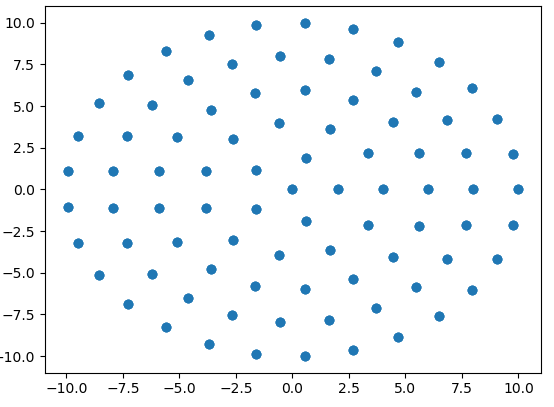
\includegraphics[width=.8\linewidth]{Zdjecia/5/siatka1}
  \caption{}
  \label{fig:sfig1}
\end{subfigure}%
\begin{subfigure}{.5\textwidth}
  \centering
  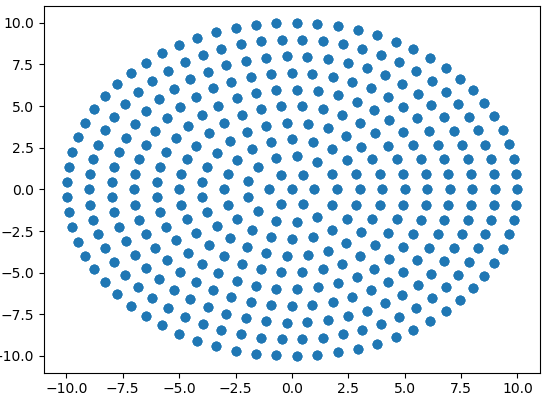
\includegraphics[width=.8\linewidth]{Zdjecia/5/siatka2}
  \caption{}
  \label{fig:sfig2}
\end{subfigure}\\
\begin{subfigure}{.5\textwidth}
  \centering
  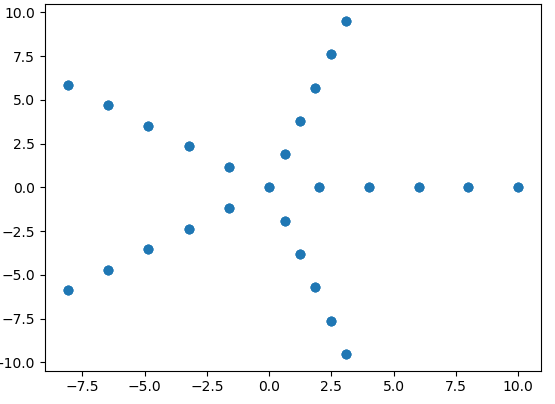
\includegraphics[width=.8\linewidth]{Zdjecia/5/siatka3}
  \caption{}
  \label{fig:sfig3}
\end{subfigure}%
\begin{subfigure}{.5\textwidth}
  \centering
  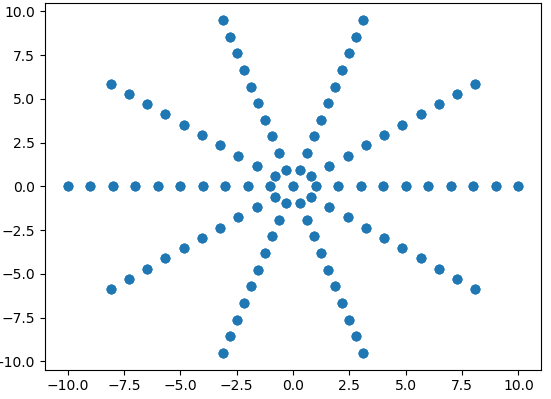
\includegraphics[width=.8\linewidth]{Zdjecia/5/siatka4}
  \caption{}
  \label{fig:sfig4}
\end{subfigure} 
\caption{Układ siatki węzłów na płaszczyźnie powstałych z a) \textit{circleMeshFull(10, 5, 5)} b) \textit{circleMeshFull(10, 10, 10)} c) \textit{circleMeshSparse(10, 10, 10)} d) \textit{circleMeshSparse(10, 10, 10)}}
\label{fig:siatka}
\end{figure}


\begin{figure}
\begin{subfigure}{.5\textwidth}
  \centering
  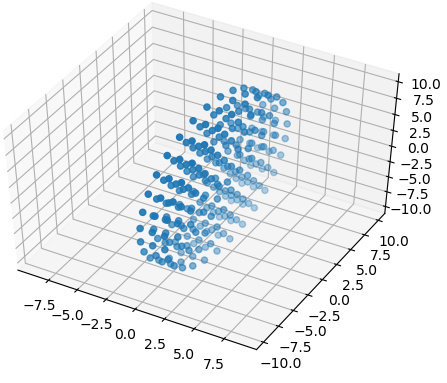
\includegraphics[width=.8\linewidth]{Zdjecia/5/pret1}
  \caption{}
  \label{fig:sfig1}
\end{subfigure}%
\begin{subfigure}{.5\textwidth}
  \centering
  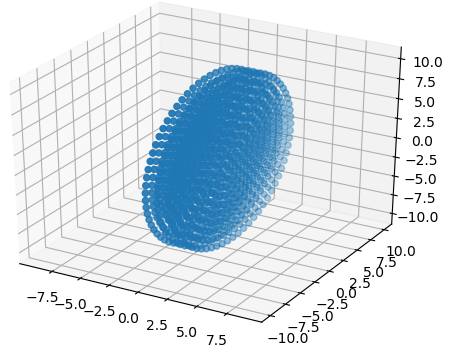
\includegraphics[width=.8\linewidth]{Zdjecia/5/pret2}
  \caption{}
  \label{fig:sfig2}
\end{subfigure}\\
\begin{subfigure}{.5\textwidth}
  \centering
  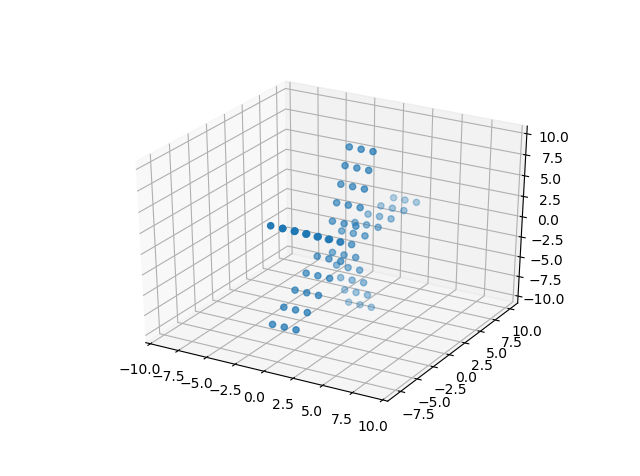
\includegraphics[width=.8\linewidth]{Zdjecia/5/pret3}
  \caption{}
  \label{fig:sfig3}
\end{subfigure}%
\begin{subfigure}{.5\textwidth}
  \centering
  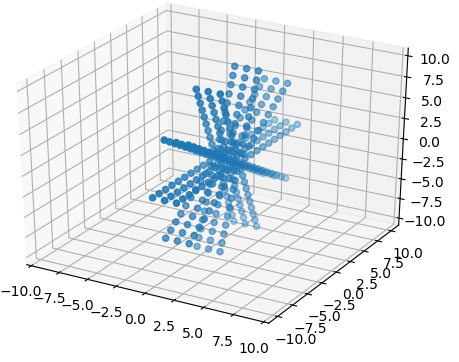
\includegraphics[width=.8\linewidth]{Zdjecia/5/pret4}
  \caption{}
  \label{fig:sfig4}
\end{subfigure} 
\caption{Układ siatki węzłów pręta z a) \textit{circleMeshFull(10, 5, 5)} b) \textit{circleMeshFull(10, 10, 10)} c) \textit{circleMeshSparse(10, 10, 10)} d) \textit{circleMeshSparse(10, 10, 10)}}
\label{fig:pret}
\end{figure}

\begin{figure}
\begin{subfigure}{.5\textwidth}
  \centering
  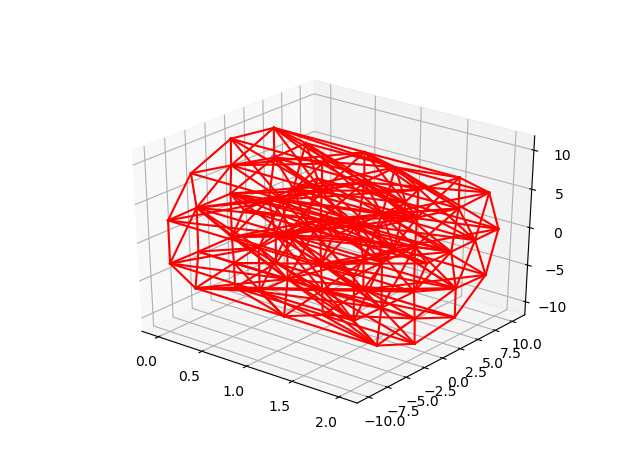
\includegraphics[width=.8\linewidth]{Zdjecia/5/triangulation1}
  \caption{}
  \label{fig:sfig1}
\end{subfigure}%
\begin{subfigure}{.5\textwidth}
  \centering
  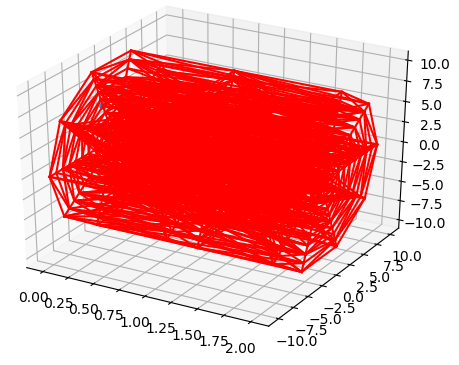
\includegraphics[width=.8\linewidth]{Zdjecia/5/triangulation2}
  \caption{}
  \label{fig:sfig2}
\end{subfigure}

\caption{Triangulacja (elementy skończone) dla siatki a) \textit{circleMeshFull(10, 3, 3)} b) \textit{circleMeshSparse(10, 10, 10)}}
\label{fig:triangulation}
\end{figure}

\vspace {3mm}
 \( \textbf{Moduł calculation4} \).

\vspace {3mm}
\textit{pVector()} - funkcja zwraca macierz zmiennych symbolicznych z wektorem p dla elementu czworościennego.

\vspace {3mm}
\textit{meMatrix(vertices, elementIndices)} - funkcja przyjmuje macierz współrzędnych węzłów - vertices oraz indeksy dla węzłów elementu skończonego - elementIndices i zwraca macierz \( M^e \).

\vspace {3mm}
\textit{meInvMatrix(vertices, elementIndices)} - jak powyżej, dodatkowo macierz wyjściowa jest odwrócona w stosunku do poprzedniej funkcji.

\vspace {3mm}
\textit{shapeFunctions(vertices, elementIndices)} - funkcja przyjmuje macierz współrzędnych węzłów - vertices i indeksy dla węzłów elementu skończonego - elementIndices, a zwraca funkcje kształtu w formie tablicy zmiennych symbolicznych.

\vspace {3mm}
\textit{bMatrixFc(shapeFunctions)} - funkcja przyjmuje tablicę funkcji kształtu w postaci symbolicznej - shapeFunctions, a zwraca macierz B w postaci tablicy numerycznej. Funkcje kształtu są dla elementów czworościennych liniowe więc ich pochodne są stałymi. 

\vspace {3mm}
\textit{bMatrixNatural(shapeFunctions)} - jak powyżej, ale dla tablicy funkcji kształtu we współrzędnych naturalnych.

\vspace {3mm}
\textit{dMatrixFc(youngModulus, poissonCoeficient)} - funkcja zwraca macierz D, obliczoną na podstawie modułu Younga - youngModulus oraz współczynnik Poissona - poissonCoeficient.

\vspace {3mm}
\textit{stiffLocalMatrix(shapeFunctions, vertices, elementIndices, youngModulus, poissonCoefficient)} - funkcja przyjmuje jako argumenty funkcje kształtu w formie symbolicznej - shapeFunctions, macierz współrzędnych węzłów - vertices, indeksy węzłów elementu skończonego - element indices oraz moduł Younga - youngModulus i współczynnik Poissona - poissonCoeficient. Zwraca macierz sztywności dla elementu skończonego.

\vspace {3mm}
\textit{massLocalMatrix(density)} - funkcja przyjmuje gęstość materiału - density. Zwraca macierz mas obliczoną we współrzędnych naturalnych bez uwzględnienia jakobianu. Na tym etapie nie jest to więc poprawnie wyznaczona macierz mas. Jakobian jest stały dla elementów czworościennych i uwzględniany jest na etapie agregacji. Pozwala to obliczyć całkę \ref{eq:macierz_mas} bez uwzględnienia jakobianu raz, a następnie mnożyć ją dla każdego elementu przez jakobian.

\vspace {3mm}
\textit{volume(elementVertices)} - funkcja przyjmuje współrzędne węzłów elementu - elementVertices i oblicza objętość elementu z wykorzystaniem geometrii analitycznej.

\vspace {3mm}
\textit{volumeDet(vertices)} - jak powyżej z tym, że objętość jest obliczano za pomocą wyznacznika macierzy \( M^e \).

\vspace {3mm}
 \( \textbf{Moduł gauss4} \).
Moduł zawiera funkcje pomocnicze do całkowania macierzy mas. Obliczanie macierzy sztywności nie wymaga całkowania, ponieważ macierz B jest stała.

\vspace {3mm}
\textit{shapeFunctionsNatural()} - zwraca tablicę funkcji kształtu we współrzędnych naturalnych, w formie symbolicznej.

\vspace {3mm}
\textit{coordinateChangeModel(elementVertices, naturalShapeFc)} - funkcja przyjmuje funkcje kształtu we współrzędnych naturalnych - naturalShapeFc  oraz współrzędne węzłów elementu skończonego - elementVertices i oblicza zależność współrzędnych rzeczywistych i naturalnych. Zwraca trzy wyrażenia symboliczne zawierające współrzędne naturalne. Przedtsawiają one współrzędne rzeczywiste, kolejno x, y, z.

\vspace {3mm}
\textit{jacobian(elementVertices, naturalShapeFc)} - funkcja przyjmuje współrzędne węzłów elementu skończonego - elementVertices oraz funkcje kształtu we współrzędnych naturalnych - naturalShapeFc. Zwraca jakobian przekształcenia, który jest wykorzystywany w obliczaniu macierzy mas.

\vspace {3mm}
\textit{matrixToIntegrate(density)} - funkcja przyjmuje gęstość materiału - density. Zwraca macierz podcałkową, do obliczania macierzy mas. Nie uwzględnia jakobianu, który jest stały. Wynik całkowania jest mnożony przez jakobian na etapie agregacji.

\vspace {3mm}
 \( \textbf{Moduł assembling4} \).
Moduł zawiera funkcje do obliczania macierzy globalnych. Pozwala też na wizualizację rzadkości macierzy.

\vspace {3mm}
\textit{assembleGlobalStiffMatrix(vertices, indices, youngModulus, poissonCoefficient)} - funkcja przyjmuje macierz współrzędnych węzłów konstrukcji - vertices, indeksy wszystkich elementów - indices, moduł Younga - youngModulus i współczynnik Poissona - poissonCoeficient. Zwraca globalną macierz sztywności.

\vspace {3mm}
\textit{drawMatrixSparsity(matrix)} - funkcja przyjmuje macierz - matrix. Pozwala rysować rzadkość macierzy w postaci bitmapy, gdzie każdy element macierzy jest jednym pikselem.

\vspace {3mm}
\textit{assembleGlobalMassMatrix(vertices, indices, density)} - funkcja przyjmuje macierz współrzędnych węzłów konstrukcji - vertices, indeksy węzłów wszystkich elementów skończonych - indices oraz gęstość materiału - density. Zwraca globalną macierz mas.

\vspace {3mm}
\textit{focuseMatrixRows(matrix)} - funkcja przyjmuje macierz - matrix. Zwraca macierz skupioną poprzez sumowanie elementów w wierszu i umieszczanie ich na diagonali. Wykorzystywana przy obliczeniach ze skupioną macierza mas.



\subsection{Elementy sześcienne}
\label{cha:elementy szescienne}

Obliczenia dotyczące elementów sześciennych zawarte są w modułach katalogu hexahedralElements. Poniżej znajdują się funkcje poszczególnych modułów, wraz z opisem ich zastosowania, argumentami wejściowymi oraz wyjściowymi.

 \( \textbf{Moduł mesh8} \).

\textit{circleMeshFull(radius, firstCircle, addNodes, circles)} - funkcja działa jak funcja z modułu mesh4 z tą różnicą, że przyjmuje dodatkowy argument addNodes. Określa on ile punktów więcej ma być na każdym kolejnym okręgu siatki.

\textit{circleMeshSparse(radius, firstCircle, circles)} - funkcja działa jak odpowiednik z modułu mesh4

\textit{createFiniteElements(vertices, pointsOnLastCircle, length, numberOfPlanes)} - funkcja przyjmuje jako argumenty macierz współrzędnych węzłów, liczbę punktów na ostatnim okręgu siatki, długość modelu pręta oraz liczbę płaszczyzn siatki. Tworzy elementy sześcienne w kilku etapach. Najpierw jedna z płaszczyzn dzielona jest na trójkąty. Następnie trójkąty są łączone w pary i w ten sposób powstają czworokąty. W większości konfiguracji siatki na brzegach pozostają puste miejsca z trójkątów, które nie mają pary. W takich miejscach dodawany jest dodatkowy punkt siatki i z trójkąta tworzony czworokąt. Następnie identyczne czworokąty są tworzone na kolejnych płaszczyznach i wzdłuż długości pręta tworzone są z nich sześciościany. Zwraca macierz e x 8, gdzie e to liczba elementów skończonych. W kolumnach są indeksy kolejnych punktów siatki.

\textit{brickMesh(radius, numberOfPlanes, numberOfCircles, numberOfPointsOnCircle)} - funkcja tworzy siatkę w kształcie wielokąta. Przyjmuje jako argumenty promień - radius, liczbę płaszczyzn siatki - numberOfPlanes, liczbę okręgów na płaszczyźnie siatki - numberOfCircles oraz ilość wierzchołków wielokąta wpisanego w okrąg - numberOfPointsOnCircle. Zwraca tablicę o wymiarach n x 3, gdzie n to liczba węzłów. W kolumnach są kolejne współrzędne węzłów.

\textit{createBrickElements(brickVertices, numberOfPlanes, numberOfCircles, numberOfPointsOnCircle)} - funkcja przyjmuje macierz współrzędnych węzłów z funkcji \textit{brickMesh} - brickVertices, liczbę płaszczyzn siatki - numberOfPlanes, liczbę okręgów na każdej płaszczyźnie - numberOfCircles oraz liczbę wierzchołków wielokąta wpisanego w każdy okrąg - numberOfPointsOnCircle. Tworzy elementy sześciościenne na zadanej siatce. Zwraca macierz e x 8, gdzie e to liczba elementów skończonych. W kolumnach są indeksy kolejnych punktów siatki.

\textit{drawPlane(vertices)} - jak w mesh4. Przykładowe siatki z tego modułu są przedstawione na rysunku \ref{fig:hex_siatka}.

\textit{drawBar(vertices)} - jak w mesh4

\textit{drawTetragons(vertices, indices)} - funkcja przyjmuje jako argumenty macierz współrzędnych węzłów - vertices oraz macierz indeksów węzłów dla każdego elementu - indices. Rysuje układ czworokątów na płaszczyźnie. Przykłady są przedstawione na rysunku \ref{fig:hex_czworokaty}.

\textit{drawHexahedrons(vertices, indices)} - funkcja przyjmuje jako argumenty macierz współrzędnych węzłów - vertices oraz macierz indeksów węzłów dla każdego elementu - indices. Rysuje model złożony z sześciościanów w rzucie izometrycznym. Przykład znajduje się na rysunku \ref{fig:hex_elementy}.

\begin{figure}
\begin{subfigure}{.5\textwidth}
  \centering
  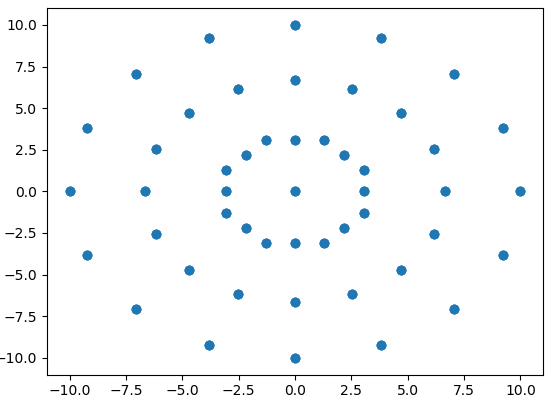
\includegraphics[width=1.0\linewidth]{Zdjecia/5/hex_siatka1}
  \caption{}
  \label{fig:sfig1}
\end{subfigure}
\begin{subfigure}{.5\textwidth}
  \centering
  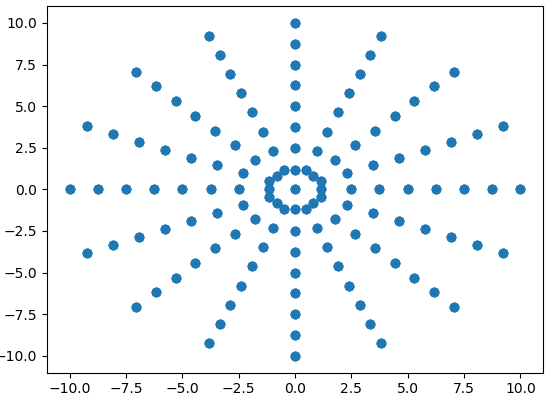
\includegraphics[width=1.0\linewidth]{Zdjecia/5/hex_siatka2}
  \caption{}
  \label{fig:sfig2}
\end{subfigure}
\caption{Układ siatki węzłów na płaszczyźnie powstałych z a) \textit{brickMesh(10, 3, 3, 16)} b) \textit{brickMesh(10, 3, 8, 16)} }
\label{fig:hex_siatka}
\end{figure}

\begin{figure}
\begin{subfigure}{.5\textwidth}
  \centering
  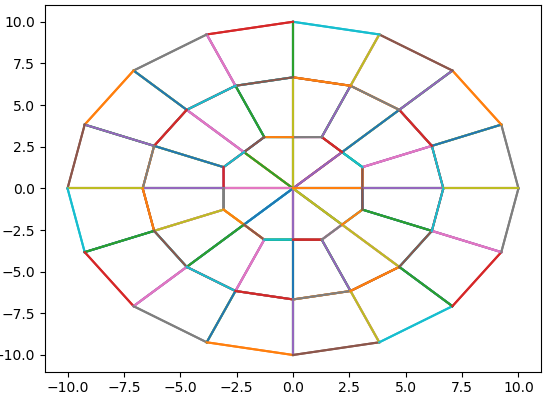
\includegraphics[width=1.0\linewidth]{Zdjecia/5/hex_czworokaty1}
  \caption{}
  \label{fig:sfig1}
\end{subfigure}
\begin{subfigure}{.5\textwidth}
  \centering
  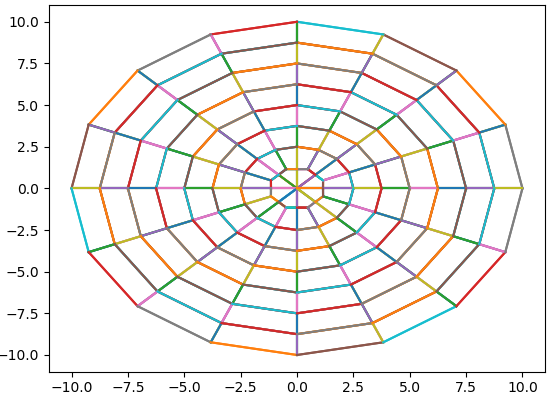
\includegraphics[width=1.0\linewidth]{Zdjecia/5/hex_czworokaty2}
  \caption{}
  \label{fig:sfig2}
\end{subfigure}
\caption{Czworokąty będące ścianą elementu skończonego na płaszczyźnie a) \textit{brickMesh(10, 3, 3, 16)} b) \textit{brickMesh(10, 3, 8, 16)} }
\label{fig:hex_czworokaty}
\end{figure}

\begin{figure}
\begin{subfigure}{.5\textwidth}
  \centering
  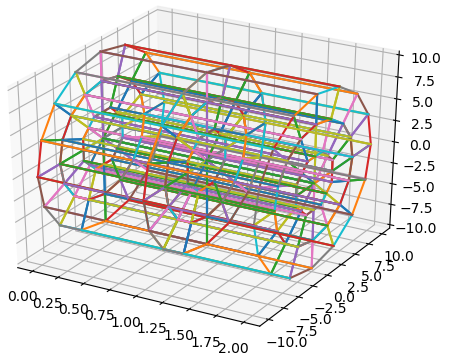
\includegraphics[width=1.0\linewidth]{Zdjecia/5/hex_elementy1}
  \caption{}
  \label{fig:sfig1}
\end{subfigure}
\begin{subfigure}{.5\textwidth}
  \centering
  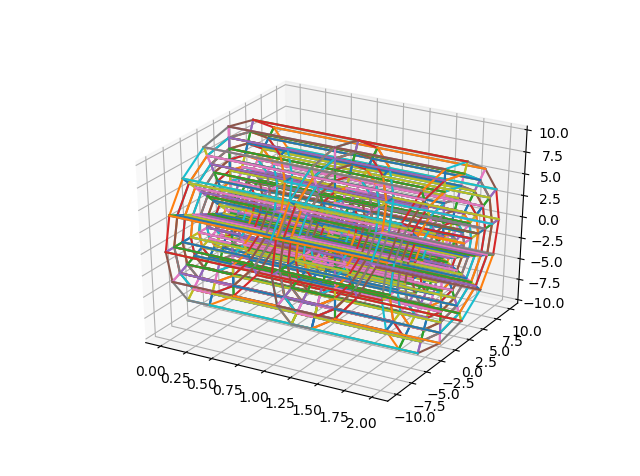
\includegraphics[width=1.0\linewidth]{Zdjecia/5/hex_elementy2}
  \caption{}
  \label{fig:sfig2}
\end{subfigure}
\caption{Elementy skończone zbudowane na siatce a) \textit{brickMesh(10, 3, 3, 16)} b) \textit{brickMesh(10, 3, 8, 16)} }
\label{fig:hex_elementy}
\end{figure}

 \( \textbf{Moduł calculations8} \).

\textit{localStiffMatrix(elementVertices)} - funkcja przyjmuje jako argumenty macierz współrzędnych węzłów elementu skończonego. Zwraca macierz sztywności elementu skończonego.

\textit{localMassMatrix(elementVertices)} - funkcja przyjmuje jako argumenty macierz współrzędnych węzłów elementu skończonego - elementVertices. Zwraca macierz mas elementu skończonego.

 \( \textbf{Moduł assembling8} \).

\textit{assembleGlobalStiffMatrix(vertices, indices)} - funkcja przyjmuje jako argument macierz współrzędnych węzłów konstrukcji - vertices oraz macierz indeksów węzłów elementów skończonych. Zwraca macierz sztywności konstrukcji.

\textit{assembleGlobalMassMatrix(vertices, indices)} - funkcja przyjmuje jako argument macierz współrzędnych węzłów konstrukcji - vertices oraz macierz indeksów węzłów elementów skończonych. Zwraca macierz mas konstrukcji.

\textit{focuseMatrixRows(matrix)} - funkcja przyjmuje macierz - matrix. Zwraca macierz skupioną poprzez sumowanie elementów w wierszu i umieszczanie ich na diagonali. Wykorzystywana przy obliczeniach ze skupioną macierza mas.

\textit{drawMatrixSparsity(matrix)} - funkcja przyjmuje macierz - matrix. Pozwala rysować rzadkość macierzy w postaci bitmapy, gdzie każdy element macierzy jest jednym pikselem.


\subsection{Pozostałe moduły katalogu MES\_dir}
\label{cha:pozostale_moduly}

 \( \textbf{Moduł config} \).

W tym module przechowywane są dane wykorzystywane w innych częściach programu. Jego zawartość podana jest poniżej.

\vspace {3mm}
ROOT\_DIR = os.path.dirname(os.path.abspath(\_\_file\_\_))

\#sciezka do katalogu MES\_dir
\vspace {3mm}
ndof = 3    \# liczba stopni swobody

kvect\_min = 0

kvect\_no\_of\_points = 0

kvect\_max = 2*pi
\vspace {3mm}
k = []  \# globalna macierz sztywnosci

m = []  \# globalna macierz mas

m\_focused\_rows = [] \#globalna macierz mas - skupiona wierszami

ml = []

m0 = []

mr = []

kl = []

k0 = []

kr = []
\vspace {3mm}
force = []
\vspace {3mm}
\# Stale materialowe

young\_mod = 70000

poisson\_coef = 0.3

density = 2.7*1e-9
\vspace {3mm}
\# Wyswietlanie siatki na plaszczyznie, siatki w 3D i triangulacji

show\_plane = False

show\_bar = False

show\_elements = False
\vspace {3mm}

Pierwszym elementem jest ścieżka do katalogu pozwalająca wygodnie odnosić się do niego w funkcjach zapisujących i wczytujących dane z plików. Poniżej znajdują się wartość minimalna, maksymalna oraz liczba próbek wartości liczby falowej, dla których to wartości obliczane będą częstości własne. Następnie kolejno zawarte są macierze i podmacierze modelu MES, siła wymuszająca wykorzystywana przy obliczaniu wzbudzalności, stałe materiałowe konstrukcji pręta i wartości logiczne określające czy wyświetlać siatkę lub element skończone modelu.

\vspace {3mm}

 \( \textbf{Moduł MES} \).
W tym module zawarte są dwie funkcje, które są przykładami budowy modelu za pomocą elementów czworościennych oraz sześciościennych.

\textit{mes4(radius, numOfCircles, numOfPointsAtFirstCircle)} - funkcja przyjmuje jako argumenty promień pręta - radius, liczbę okręgów na jednej płaszczyźnie siatki - numOfCircles oraz liczbę węzłów na pierwszym okręgu siatki - numOfPointsAtFirstCircle. Poniżej znajduje się całość kodu tej funkcji.

\vspace {3mm}

    vertices = mesh4.circleMeshFull(radius, numOfCircles, numOfPointsAtFirstCircle)

    if config.show\_plane:

        mesh4.drawPlane(vertices)

    if config.show\_bar:

        mesh4.drawBar(vertices)

\vspace {3mm}
    indices = mesh4.triangulation(vertices)

    \# mesh.draw\_triangulation(vertices, indices)

    if config.show\_elements:

        mesh4.drawTriangulation(vertices, indices)

\vspace {3mm}
    start = time.clock()

    config.k = assembling4.assembleGlobalStiff\_matrix(vertices, indices, config.young\_mod, config.poisson\_coef)

    \# assembling.drawMatrixSparsity(config.k)

    print("Macierz sztywnosci gotowa")

    print("Wykonywanie: ", time.clock() - start)

\vspace {3mm}
    config.m = assembling4.assembleGlobalMassMatrix(vertices, indices, config.density)

    config.m\_focused\_rows = assembling4.focuseMatrixRows(config.m)

    \# assembling.drawMatrixSparsity(config.m)

    print("Macierz mas gotowa")

    print("wykonywanie: ", time.clock() - start)

\vspace {3mm}

W pierwszej lini uzyskiwana jest macierz współrzędnych węzłów siatki. Następnie siatka jest wyświetlana w na płaszczyźnie, bądź w rzucie izometrycznym jeśli wartości z modułu config mają wartości TRUE. Kolejnym etapem jest tworzenie elementów skończonych i warunkowe ich wyświetlanie. Wartość start przechowuje czas, w którym rozpoczyna się obliczanie macierzy sztywności - k. Po obliczeniu tej macierzy wyświetlany jest komunikat z czasem obliczeń.  Podobnie poniżej w przypadu macierzy mas.

\textit{mes8(numberOfPlanes, radius, numberOfCircles, numberOfPointsOnCircle, addNodes)} - funkcja przyjmuje jako argumenty liczbę płaszczyzn siatki - numberOfPlanes, promień pręta - radius, liczbę okręgów na jednej płaszczyźnie siatki - numOfCircles, liczbę węzłów na pierwszym okręgu siatki - numOfPointsOnCircle oraz liczbę dodatkowych punktów na każdym kolejnym okręgu siatki przy zastosowaniu odpowiedniego jej typu - addNodes. Poniżej znajduje się całość kodu tej funkcji.

\vspace {3mm}
    \# brickMesh(radius, numberOfPlanes, numberOfCircles, numberOfPointsOnCircle)

    vertices = mesh8.brickMesh(radius, numberOfPlanes, numberOfCircles, numberOfPointsOnCircle)

    \# createBrickElements(brickVertices, numberOfPlanes, numberOfCircles, numberOfPointsOnCircle)

    indices = mesh8.createBrickElements(vertices, 3, 3, 16)

\vspace {3mm}
    start = time.clock()

    config.k = assembling8.assembleGlobalStiffMatrix(vertices, indices)

    print("Macierz sztywnosci gotowa")

    print("Wykonywanie: ", time.clock() - start, " [s]")

    print("Wykonywanie: ", (time.clock() - start)/3600, " [h]")

    start = time.clock()

\vspace {3mm}
    config.m = assembling8.assembleGlobalMassMatrix(vertices, indices, config.density)

    config.m\_focused\_rows = assembling8.focuse\_matrix\_rows(config.m)

    print("Macierz mas gotowa")

    print("wykonywanie: ", time.clock() - start, " [s]")

    print("wykonywanie: ", (time.clock() - start)/3600, " [h]")

\vspace {3mm}
W tym przykładzie zastosowano siatkę brickMesh. Po wyznaczeniu współrzędnych węzłów oraz zbudowaniu elementów skończonych, obliczane są macierze mas i sztywności.

 \( \textbf{Moduł dispersion\_curves} \).
W tym module wyznaczone są punkty krzywych dyspersji, na podstawie macierzy mas i sztywności wyznaczonych z modelu MES.

\vspace {3mm}
\textit{getDataForEiq()} - funkcja wyznacza podmacierze mas i sztywności potrzebne do zastosowania wzoru \ref{eq:MES5}. Macierze przechowywane są w module \textit{config}. Dodatowo po wyznaczeniu zapisywane są do plików tekstowych, tak więc nie ma potrzeba wyznaczania ich ponownie w celu innego wykorzystania.

\vspace {3mm}
\textit{findEig()} - funkcja dla kolejnych wartości liczby falowej oblicza wartości i wektory własne pary macierzy, wyznaczonych jak we wzorze \ref{eq:MES5}. Dodatkowo wektory własne zapisywane są w niej do pliku.

\vspace {3mm}
\textit{drawDispercionCurves(number\_of\_curves\_to\_draw=10, save\_plot\_to\_file=False)} - funkcja przyjmuje jako argument liczbę początkowych modów do wyświetlenia - number\_of\_curves\_to\_draw oraz wartość logiczną określająca czy zapisać wykres do pliku png - save\_plot\_to\_file. Dodatkowo zapisauje wszystkie wartości własne w pliku tesktowym.

\vspace {3mm}
\textit{drawDispercionCurvesFromFile(number\_of\_curves\_to\_draw=10, save\_plot\_to\_file=False)} - jak powyżej z tym, że funkcja ta służy do rysowania krzywych dyspersji z wartości wczytywanych z plików tekstowych.

\vspace {3mm}
\textit{sortColumns(matrix)} - funkcja służy do wstępnego sortowania wartości własnych. Sortuje je kolumnami od najmniejszej do największej. W każdej kolumnie zapisane są wartości własne dla jednej wartości liczby falowej. Sortowanie takie jest więc poprawne tylko dla modów początkowych, które się nie krzyżują. Bardziej zaawansowany algorytm sortowania jest wprowadzany na etapie obliczeń związanym z wykorzystywaniem krzywych dyspersji.

\vspace {3mm}
 \( \textbf{Moduł excitabiliti\_curves} \).
Moduł pozwala na obliczanie krzywych wzbudzalności dla poszczególnych modów. 

\vspace {3mm}
\textit{hermitianTranspose(matrix)} - funkcja przyjmuje jako argument macierz, a zwraca sprzężenie hermitowskie macierzy wejściowej.

\vspace {3mm}
\textit{calculateP(kr, kl, wavenumber, eigvector)} - funcja przyjmuje jako argumenty podmacierze macierzy sztywności \( k\_r \) i \(k\_l \) wykorzystywane wcześniej we wzorze \ref{eq:MES5}, wartości liczby falowej, dla których wyznaczano wartości i wektory własne - wavenumber oraz wektory własne - eigvector. Zwraca wartość \( P \) zgodnie ze wzorem \ref{eq:wzbudzanie3}.

\vspace {3mm}
\textit{calculateExcitablity(mode, f)} - funkcja przyjmuje jako argumenty numer modu - mode oraz wektor będący wymuszającą siłą węzłową dla modelu MES - f. Wyznacza dla każdej częstotliwości, z którą związany jest wektor własny, wartość amplitudy. Zwraca wektor częstotliwości i amplitudy.

\vspace {3mm}
\textit{calculateAndShowCurves(numberOfModes)} - funkcja przyjmuje jako argument liczbę początkowych modów, dla których ma wyznaczyć krzywe wzbudzalności- numberOfModes. Po obliczeniu przedstawia wykres krzywych wzbudzalności.

\vspace {3mm}
 \( \textbf{Moduł readData} \).
W tym module zawarte są wszystkie funkcje służące do zapisu i wczytywania danych. Nie będą one z osobna omawiane ponieważ ich funkcja jest jasna. Poniżej omówiony jest sposób umieszczania danych w plikach.

Wszystkie dane umieszczone są w katalogu \textit{eig}. Liczby falowe zapisane są w pliku \textit{kvect}. Każda wartość znajduje się w osobnej lini.

Wartości własne zapisane są w katalogu \textit{eig} w pliku \textit{omega}. Każda kolumna zawiera wartości wyznaczone dla jednej wartości liczby falowej.

Wektory własne zapisywane są w katalogu \textit{eig}, w plikach mających w nazwie \textit{eig\_}, a następnie wartość liczby falowej. W każdym z takich plików zapisane są wartości własne i odpowiadające im wektory własne dla jednej wartości liczby falowej. W pierwszej linii znajduje się wartość własna, w drugiej odpowiadający jej wektor własny, a następnie pozostałe wartości i wektory własne w kolejnych liniach.

\subsection{Moduł main}
\label{cha:main}

Przykładowy skrypt wyznaczający krzywe dyspersji, z pomocą wcześniej opisanych modułów, znajduje się w module \textbf{main} głównego katalogu projektu. Kod przedstawiony jest poniżej.

\vspace{3mm}
import sympy as sp

import numpy as np

from MES\_dir import MES, config, dispersion\_curves

from MARC import functions

\vspace{3mm}
\# begin MES

x, y, z = sp.symbols('x, y, z')

if \_\_name\_\_ == "\_\_main\_\_":

\vspace{3mm}
    print("Wpisz wartość: ")

    print("1 - rysowanie krzywy dyspersji z wykorzystaniem MES")

    print("2 - rysowanie krzywych dyspersji z ostatnio policzonych danych")

    text = input()

\vspace{3mm}
    if text == '1':

\vspace{3mm}
        print("Wpisz wartość: ")

        print("4 - elementy czworościenne")

        print("8 - elemnty sześcienne")

        print("M - wczytanie macierzy z MARC i wykreślenie krzywych")

        text1 = input()

\vspace{3mm}
        \# wektor liczby falowej

        config.kvect\_min = 1e-10

        config.kvect\_max = np.pi / 4

        config.kvect\_no\_of\_points = 51

\vspace{3mm}
        \# rysowanie wykresow

\vspace{3mm}
        config.show\_plane = True

        config.show\_bar = True

        config.show\_elements = True

\vspace{3mm}
        \# obliczenia

        if text1 == '4':

            \# parametry preta

            radius = 10

            num\_of\_circles = 4

            num\_of\_points\_at\_c1 = 4

            MES.mes4(radius, num\_of\_circles, num\_of\_points\_at\_c1)

\vspace{3mm}

        if text1 == '8':

            radius = 10

            numberOfPlanes = 3

            firstCircle = 16 \#for brickMesh should be 16

            addNodes = 0

            circles = 1

            MES.mes8(numberOfPlanes, radius, circles, firstCircle, addNodes)

\vspace{3mm}
        if text1 == 'M':

            config.k, config.m = functions.getStiffAndMassMatrix()

        dispersion\_curves.drawDispercionCurves()

        print("koniec")

\vspace{3mm}
    \# rysowanie krzywych dyspersji z wczesniej obliczonych wartosci

    if text == '2':

        dispersion\_curves.drawDispercionCurvesFromFile()

\vspace{3mm}
Pierwsze linijki zapewniają dostęp do funkcji z potrzebnych modułów programu oraz bibliotek Python-a. Następnie znajduje się definicja zmiennych symbolicznych, które są wykorzystywane w programie. W dalszej części następuje seria warunków, które pozwalają na wybor obliczania nowych wartości własnych (text=1), bądź skorzystana z wcześniej wyznaczonch do wykreślenia krzywych dyspersji (text=2). Wyboru dokonujemy poprzez wpisane odpowiedniej cyfry w konsoli programu. 

Jeśli chcemy obliczyć nowe krzywe, to będziemy mogli skorzystać z budowania modelu MES przy pomocy elementów czworościennych (text1=4), elementów sześciennych (text1=8), bądź skorzystać z modelu wyznaczonego w programie MARC (text1=M) i zapisanego w postaci plików z roszerzeniem dat w katalogu \textit{MARC}. Niezależnie od wybranego sposobu dostarczania modelu, program w kolejnej fazie przejdzie do wyznaczania krzywych dyspersji.

Siatkę dla elementów skończonych możemy dostosować przez zmianę odpowiednich wartości przyjmowanych jako argumenty funkcji \textit{mes4} oraz \textit{mes8}. Dla zmiany rodzaju siatki należy wybrać inną funkcję do jej generacji w funkcji \textit{mes4} lub \textit{mes8}. Należy przy tym pamiętać żeby dostosować także funkcję budującą elementy skończone. Przykładowo dla siatki tworzonej przy pomocy \textit{brickMesh}, powinna to być funkcja \textit{createBrickElements}.





\section{Segregacja krzywych dyspersji}
Kod odpowiedzialny za segregację krzywych dyspersji wygenerowanych z solvera opisanego w poprzedniej sekcji znajduje się w pliku selectMode.py w katalogu o nazwie Propagation. Jego miejsce w drzewie projektu przedstawia rysunek \ref{fig:gdzie jest select}
\begin{figure}[h]
\centering
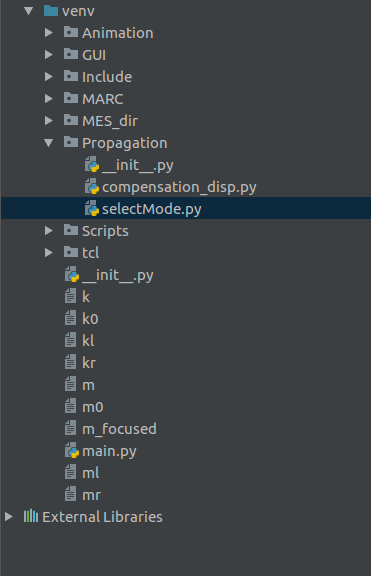
\includegraphics[width=10cm]{Zdjecia/5/kasia/selectMode}
\caption{Lokalizacja pliku selectMode.py w drzewie projektu}
\label{fig:gdzie jest select}
\end{figure}
Jest to jedyna część aplikacji napisana całkowicie obiektowo. Zastosowanie programowania obiektowego w przypadku tej części aplikacji znacząco ułatwiło późniejsze używanie stworzonego rozwiązania jak i uporządkowało sam kod. Plik selectMode został stworzony aby w sposób łatwy i szybki można było przeprowadzić agregacją punktów do konkretnych krzywych dyspersji a następnie w sposób łatwy i intuicyjny z nich korzystać. Samo generowanie obiektu przechowującego wszystkie krzywe dyspersji jest bardzo łatwe. Należy najpierw stworzyć obiekt typu SelectMode, jako argumenty podając ścieżki względne kolejno do pliku kvect oraz omega. Następnie należy wywołać metodę stworzonego właśnie obiektu o nazwie selectMode(). Od tego momentu nasz obiekt przechowuje posortowane krzywe dyspersji.

Podstawową jednostką są tu obiekty klasy Point. Klasa ta jak wszystkie omawiane w tej sekcji znajduje się w pliku selctMode.py. Klasa ta posiada jedynie konstruktor, przyjmujący dwa parametry: w,k. Obiekt ten reprezentuje pojedynczy punkt wygenerowany przez zaimplementowany solver MES. Wartość w jest wartością zespoloną i odpowiada wartości znajdującej się na osi x wykresu krzywej dyspersji, czyli częstości kątowej, natomiast k odpowiada wartości y tego wykresu i oznacza liczbę falową. Obydwa parametry przyjmują wartości domyślne wynoszące zero. Klasa ta ma cztery pola:

$w$ - przechowujące wartość częstotliwości w kHz

$wkat_real_part$ - przechodujące część rzeczywistą podanej do konstruktora częstości

$wkat_complex$ - przechowujące zespoloną częstość kątową podaną do konstruktora

$k$ - przechowujące wartość liczby falowej podaną do konstruktora.

Klasa ta posiada tylko jedną metodę:

$printCoor()$, która nie przyjmuje żadnych argumentów. Jej funkcją jest wypisywanie w konsoli współrzędnych punktu w postaci: "w=[wartość w kHz], k=[wartość w rad/m]"

Kolejną, bardziej złożoną klasą, wykorzystywaną do przechowywania krzywych dyspersji jest klasa $Mode$. Jej głównym zadaniem jest przechowywanie zbioru punktów. Posiada konstruktor bezparametrowy oraz następujące pola:

$points$ - tablica przechowująca zbiór punktów, domyślnie pusta

$minOmega$ - minimalna przechowywana wartość $\omega$ wyrażona w kHz, póki tablica $points$ jest pusta przyjmuje wartość $float('inf')$

$min_omega_kat$ = minimalna przechowywana wartość $\omega$ wyrażona w $\frac{rad}{s}$, póki tablica $points$ jest pusta przyjmuje wartość $float('inf')$

$allOmega$ - tablica przechowująca wartości wszystkich częstotliwości w postaci zespolonej, domyślnie pusta

$all_omega_khz$ - tablica przechowująca wartości wszystkich częstotliwości w kHz, domyślnie pusta

Klasa ta ma zaimplementowane następujące metody:

$addPoint$ funkcja ta przyjmuje jeden parametr. Jest nim obiekt klasy Point. Dodaje ona punkt do listy punktów ($self.points$), list $self.allOmega$ i $self.all)omega)khz$ oraz, jeśli to konieczne ustawia wartości pól $self.min_omega_kat$ oraz $minOmega$.

$delPoint$ funkcja analogiczna znaczeniowo do $self.addPoint$, jako parametr przyjmuje obiekt klasy Point. Podany punkt jest wyszukiwany w tablicy $self.points$ a następnie usuwany.

$delDuplicats$ funkcja przyjmująca jako argument tablice obiektów typu Point. Jej zadaniem jest usunięcie z tablisy $self.points$ wszystkich punktów z podanej listy.

$quicksort$ to funkcja przyjmująca dwa parametry, indeks początkowy i końcowy. Jej zadaniem jest posortowanie przechowywanych punktów rosnąco względem częstości kątowych. Argument $pocz$ oznacza początkowy indeks tablicy, natomiast $koniec$ indeks końcowy. Jest to funkcja działająca rekurencyjnie. Zasada działania tego sortowania opiera się na metodzie "dziel i zwyciężaj", której główną zasadą jest rozbijanie dużego problemu na skończoną ilość mniejszych podproblemów tak długo, aż staną się one trywialne do rozwiązania. W tym przypadku wybiera się tak zwany piwot wokół którego rozdziela się elementy do lewej i prawej tablicy. W lewej znajdują się elementy mniejsze w prawej większe. W ten sposób piwot znajduje sia na swoim właściwym miejscu. Natomiast na lewej i prawe tablicy znów wywołuje się metode quicksort. Postępuje się w ten sposób aż do uzyskania tablic jednoelementowych, które są już posortowane. Jest to bardzo dobry algorytm, zwłaszcza do sortowania dużej ilości danych.

$findAngle$ to funkcja przyjmująca jeden parametr - obiekt typu Point. Ma ona za zadanie wyznaczyć kąt pomiędzy dwoma wektorami. Pierwszy z nich stworzony jest przez dwa ostatnie punkty w tablicy $self.points$ drugi natomiast to wektor mający początek w ostatnie punkcie tablicy $self.point$ natomiast koniec w podanym w argumencie punkcie. Do obliczenia szukanego kąta wykorzystywana jest następująca zależność:
\begin{equation}
cos \alpha = \frac{a \circ b}{|a|\cdot |b|}
\end{equation}
\begin{equation}
\alpha = arccos \frac{a \circ b}{|a|\cdot |b|}
\end{equation}

Gdzie:
$a \circ b$ - oznacza iloczyn skalarny wektorów a i b

$|a|,|b|$ - oznacza długość tych wektorów

Funkcja zwraca wartość tak obliczonego kąta.

$findSmallestAngle$ jest funkcją przyjmującą dwa argumenty. Pierwszy z nich to jednowymiarowa tablica obiektów klasy Point, natomiast drugi do odległość wyrażona w kHz, w jakiej mają znajdować się brane pod uwagę punkty. Funkcja bierze wszystkie punkty z podanej listy i wybiera spośród nich ten, który tworzy najmniejszy kąt z wektorem stworzonym z dwóch ostatnich punktów. Brane pod uwagę są tylko te punkty, które znajdują się odpowiednio blisko ostatniego punktu listy $self.points$. wartość drugiego parametru jest ustawiona na domyślną. Jeśli w trakcie przeszukiwania danej tablicy punktów okazałoby się, że nie ma punktu w wyznaczonym otoczeniu, funkcja wywoływana jest rekurencyjnie z odpowiednio powiększonym zakresem otoczenia. Wartość zwracana to indeks punktu, najlepiej pasującego do już istniejącego zbioru punktów. Funkcja ta jest wykorzystywana bezpośrednio do segregacji krzywych dyspersji. Znalezienie punktu najbardziej odpowiadającego już istniejącej krzywej, a co za tym idzie tworzącego najmniejszy kąt i znajdującego się w odpowiednim sąsiedztwie jest kluczowym zadaniem pozwalającym na segregację punktów.

$findPointWithK$ przyjmuje jeden argument, k. Wyszukuje w tablicy $self.points$ wszystkie punkty, których wartość pola k jest równa zadanej wartości. Zwraca tablicę tych punktów.

$findPoint$ przyjmuje dwa argumenty: points i omega. Points to dwuelementowa tablica zawierająca obiekty klasy Point. Funkcja na podstawie podanych dwóch punktów interpoluje prostą iraz zwraca wartość tej prostej w punkcie omega.

$findPointWithGivenK$ przyjmuje dwa argument: points oraz k. działa analogicznie do funkcj $self.findPoin$ lecz zamiast zwracać wartość funkcji na podstawie jej argumentu, zwraca argument na podstawie podanej wartości k, zwracana wartość wyrazona jest w kHz.

$findPointWithGivenK_rad_s$ ta funkcja również przyjmuje dwa argumenty, a jej działanie jest identyczne jak działanie funkcji self.findPointWithGivenK, z tą różnicą, iż zwracany wynik wyrażony jest w $\frac{rad}{s}$

$findKWithGivenOmega_kHz$ przyjmuje jeden parametr, omega, będący częstotliwością wyrażoną w kHz. Oblicza wartość przechowywanej krzywej dyspersji dla podanej częstotliwości. Zwraca liczbę falową odpowiadającą podanej omedze.

Klasa Mode wykorzystywana jest zarówno do przechowywania zbioru punktów (na początek przechowuje cały zbiór wygenerowanych przez solver punktów), jak również na późniejszym etapie obiekty typu Mode przechowują pojedyncze krzywe dyspersji.

Kolejną klasą w stworzonej strukturze jest klasa Data. Posiada ona konstruktor bezparametrowy oraz jedno pole:

$modeTable$ - jest to tablica przechowująca obiekty typu Mode, przechowujące punkty należące do kolejnych krzywych dyspersji.

Klasa ta posiada również jedną metodę:

$addMode$ - przyjmuje obiekt typu mode i dodaje go do tablicy $self.modeTable$

Najbardziej nadrzędną klasą jest klasa SelectMode. Posiada ona konstruktor przyjmujący trzy parametry: 

$kvect_path$ - ścieżka do wygenerowanego przez solver pliku kvect, 

$omega_path$ - ścieżka do wygenerowanego przez solver pliku omega, 

$rows$ - liczba kolumn w pliku omega, które chcemy wczytać, domyślnie ustawiona na cały plik czyli 426 kolumn.

Klasa ta posiada 5 pól. Są to:

$eig_path$ - przechowująca podaną ścieżkę do pliku kvect

$omega_path$ - przechowująca podaną ściężkę do pliku omega

$rows$ - przechowująca liczbę kolumn do odczytu

$AllModes$ - obiekt typu Data. Na poczatku nie przechowujący żadnych danych

$k_v$ - wektor wartości liczby falowej. Domyślnie pusty

W klasie tej zostały zaimplementowane trzy metody:

$getMode$, która jako argument przujmuje liczbę całkowitą, natomiast zwraca obiekt typu Mode. Jej zadaniem jest z obiektu przechowującego wszystkie krzywe dyspersji, wybrać tę o podanym numerze i zwrócić ją w postaci obiektu klasy Mode.

$plot_modes$, która jako argument przyjmuje tablice liczb całkowitych będących indeksami krzywych, które chcemy wyświetlić. Ta funkcja niczego nie zwraca, jedynie generuje wykres żądanych krzywych dyspersji.

$selectMode$ jest funkcją nie przyjmującą żadnych parametrów. Na podstawie podanych do konstruktora danych wczytuje wektor liczb falowych z pliku kvect. następnie tworzy obiekt typu Mode,$AllPoints$, do którego następnie wczytuje wszystkie punkty wygenerowane przez solver. Następnie tworzone są dwa obiekty klasy Mode: $MinKTable$ oraz $MinKTable2$ Pierwsza z nich przechowuje punkty o wartości k równej najmniejszej wartości występującej w wektorze liczb falowych, natomiast druga przechowuje punkty, których wartość liczby falowej jest drugą najmniejszą wartością z wektora liczb falowych.

Te wybrane punkty, uszeregowane względem omeg stanowią zestaw dwóch pierwszych punktów kolejnych krzywych dyspersji. Następnym krokiem jest usunięcie ich z wektora $self.AllPoints$. Ostatnim etapem segregacji jest wybieranie kolejnych punktów z wektora $self.AllPoints$ o aktualnie najniższej wartości liczby falowej, oraz przydzielanie ich do odpowiednich modów, używając funkcji $findSmallestAngle$. Wszystkie przydzielone punkty są usuwane z wektora $self.AllPoints$. Procedura jest powtarzana do momentu aż wektor ten stanie się pusty.

Listing przykładowego kodu, agregującego punkty do krzywych dyspersji, oraz rysowania wybranej krzywej:

$Mody = SelectedMode('../eig/kvect', '../eig/omega')$

$Mody.selectMode()$

$Mody.plot_modes(50)$



\section{Metody kompensacji dyspersji}

Wszystkie zaimplementowane metody związane z kompensacją dyspersji znajdują się w pliku $compensation\_disp.py$ w folderze Propagation. Lokalizację pliku przedstawia rysunek \ref{fig:compensation}
\begin{figure}[h]
\centering
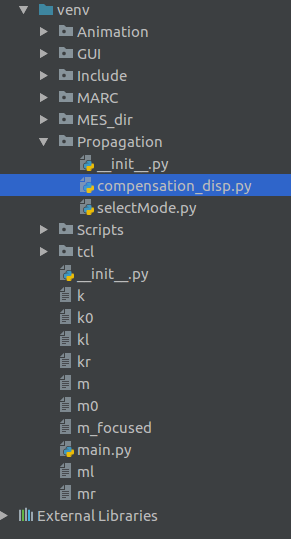
\includegraphics[width=8cm]{Zdjecia/5/kasia/compensation}
\caption{Lokalizacja pliku $compensation\_disp.py$ w drzewie projektu}
\label{fig:compensation}
\end{figure}

Trzy podstawowe metody znajdujące się w tym pliku odpowiadają trzem opisanym wcześniej metodom kompensacji. Są to:

$linear\_mapping\_compensation(signal, number\_of\_modes, disp\_curves)$ funkcja kompensująca dyspersję przy pomocy liniowego przybliżenia szeregu Taylora, opisana w rozdziale 4.4. Funckja przyjmuje trzy argumenty. Pierwszy z nich , $signal$, jest dwuelementową tablicą reprezentującą sygnał, który ma zostać skompensowany. $signal[0]$ to wektor czasu tego sygnału, natomiast $signal[1]$ to wektor wartości sygnału w kolejnych chwilach czasowych. Konwencja przechowywania sygnału w postaci dwuelementowej tablicy jest zachowana w calym pliku. Kolejnym przyjmowanym argumentem, $number\_of\_modes$, jest to liczba całkowita, będąca indeksem krzywej dyspersji, która powinna zostać użyta do kompensacji dyspersji. ostatnim argumentem, $disp\_curves$, jest obiekt klasy $SelectedMode$ przechowującym zaagregowane krzywe dyspersji. wartością zwracaną jest skompensowany sygnał w postaci dwuelementowej tablicy $[wektor\_czasu, wektor\_wartości]$.

$time\_reverse\_compensation(signal, distance, numbers\_of\_modes, disp\_curves)$ funckja generująca sygnał, którego zadaniem jest skompensowanie się na zadanej odległości przy założeniu propagacji wybranych trybów fali. Metoda ta opisana została w rozdziale 4.3. Funkcja przyjmuje cztery parametry. Pierwszy z nich, $signal$ jest sygnałem, który użytkownik chce otrzymać po propagacji. Jego format jest analogiczny jak w poprzednio omawianej funkcji. Kolejny argumentem jest $distance$. Jest to liczba, wyrażająca w metrach odległość po jakiej sygnał powinien się skompensować. Następny argument to $numbers\_of\_modes$. Jest to jednowymiarowa tablica liczb całkowitych. Zawiera ona indeksy krzywych dyspersji, tych postaci fali, które mają propagować w pręcie. Funckja zwraca sygnał, który przepropagowany przez pręt, o zadaną odległość sam się skompensuje. Ostatnim argumentem jest obiekt przechowujący krzywe dyspersji.

$mapping\_from\_time\_to\_distance(dispersion, dispercion\_curves,$
$ propagated\_modes, need\_to\_pad = False)$ jest funkcją kompensującą rozproszony sygnał przy pomocy mapowania funkcji w dziedzinie czasu na dziedzinę odległości, opisaną w rozdziale 4.5. Przyjmuje cztery argumenty w tym ostatni jest argumentem o wartości domyślnej równej False. Pierwszy z nich $dispersion$ jest sygnałem, który należy skompensować. Drugi argument to obiekt, przechowujący krzywe dyspersji. Następnie jednowymiarowa tablica liczb całkowitych, przekazująca do funkcji indeksy postaci fali, które propagowały  wbadanym obiekcie. Ostatni parametr jest opcjonalny. Domyślnie przyjmuje on wartośći False. W aplikacji funkcja generująca przepropagowany sygnał zapewnia jego wydłużenie poprzez dodanie zer. Z tego powodu domyślnie argument ten jest ustawiony na wartość False. Jeśli jednak wyniki z funkcji nie dają dobrych rezultatów, powstały sygnał nie jest skompnensowany. Należy ustawić te flagę na wartość True. Funkcja zwraca dwuelementową tablicę w postaci $[wektor\_odległości, wartości\_funkcji]$

\textbf{Pozostałe funkcje zawarte w pliku} są używane przez zaprezentowane już funkcje. Są to:

$find\_accurate\_len(actual\_len, factor=8)$ - jest to funkcja, która znajduje porządaną długość wektora. Jak zostało to napisane w [\textcolor{red}{Wilcox}], najlepiej aby sygnał wyłożony zerami po wydłużeniu miał liczbę próbek równą jakiejś potędze dwójki. Pierwszy argument to obecna długość sygnału, natomiast drugi parametr, przyjmujący domyślnie wartość 8 mówi ile razy użytkownik chce wydłużyć sygnał. Funkcja zwraca długość sygnału o długości, która jest potęgą dwójki nie mniejszą od pierwotnej długości pomnożonej przez współczynnik $factor$.

$pad\_timetraces\_zeroes(time\_vector, signal\_vector, multi=8)$ - funkcja, której zadaniem jest uzupełnić podany sygnał odpowiednią ilością zer. Pierwszym argumentem jest wektor czasu sygnału, drugim wartości sygnału w czasie. Ostatnim przekazywanym parametrem jest liczba całkowita, mówiąca ile razy chcemy wydłużyć podany sygnał. Domyślnie przyjmuje wartość 8. Wartość parametru $multi$ jest przekazywana do funkcji $find\_accurate\_len$ jako argument $factor$. Funckja zwraca sygnał wyłożony w formacie $[wydłużony\_wektor\_czasu, wartości\_wydłużonego\_sygnału]$

$calculate\_n(k\_Nyquista, delta\_k, factor=1.1)$ - funkcja obliczająca wartość n zgodnie ze wzorem 4.35. Przyjmowane przez nią argumenty to liczba falowa Nyquista, krok liczby falowej oraz współczynnik, który domyślnie przyjmuje wartość 1.1. Ponieważ nierówność 4.35 jest ostra, współczynnik ten musi być większy od 1. W przypadku podania do funkcji wartości mniejszej niż 1 wartość ta zostanie automatycznie ustawiona na 1.1. Wartością zwracaną jest wartość liczby n spełniającą wymaganą nierówność

$calculate\_k\_nyquist(dispercion\_curves, dt, factor=1.1)$ - funkcja obliczająca wartość liczby falowej Nyquista. Korzystający z nierówności 4.34. Jako argumenty przyjmuje obiekt zawierający krzywe dysperji, krok czasowy oraz współczynnik, który domyślnie przyjmuje wartość 1.1. Tak jak w przypadku poprzedniej funkcji, w przypadku podania wartości mniejszej od 1 zostanie ona ustawiona na wartość domyślną, tak samo jak w przypadku nie podania wartości tego argumentu. Wartościa zwracaną, jest wyliczona wartość liczby falowej Nyquista.

$calculate\_delta\_k(max\_v\_gr, signal\_duration, factor=0.9)$ - funkcja wyliczająca potrzebny krok liczby falowej zgodnie z zależnością 4.33. Jako argumenty przyjmuje maksymalną prędkość grupową, długość trwania sygnału oraz współczynnik. Ostatni argument ma wartość domyślną równą 0.9. Wynosi ona tyle zarówno w przypadku, gdy argument nie zostanie podany jawnie do funkcji jak i w przypadku w którym podana wartość będzie większa lub równa 1. Wartością zwracaną jest obliczona wartość $\Delta k$

$calculate\_delta\_x(k\_Nyquista)$ - funkcja wyliczająca wartość $\Delta x$. Jako parametr przyjmuje liczbę falową Nyquista natomiast zwraca obliczoną wartość $\Delta x$

$find\_max\_k(mode, k\_vect, max\_omega\_kHz)$ - funkcja pobiera jako argumenty, obiekt klase Mode, reprezentujący wybraną krzywą dyspersji, wektor liczb falowych oraz wartość częstotliwości. Na ich podstawie oblicza wartość krzywej dyspersji i ją zwraca. Funkcja ma na celu znalezienie wartości liczby falowej dla największej wartości częstotliwości występującej w sygnale wzbudzającym. W przypadku, w którym podana częstotliwość nie wzbudzi rządanej postaci. Funkcja zwróci wartość -1

$find\_omega\_in\_dispercion\_curves(mode, temp\_k, k\_vect)$ - metoda przyjmująca trzy argumenty: obiekt klasy Mode, reprezentujący krzywą dyspersji, wartość na krzywej dyspersji dla której chcemy odnaleźć odpowiadającą częstotliwość oraz wektor liczb falowych. Na podstawie podanej wartości liczby falowej obliczana jest poszukiwana wartość częstotliwości. Wartość zwracana jest poszukiwaną wartością wyrażoną w kHz.

$find_omega_in_dispercion_curves_rad_s(mode, temp_k, k_vect)$ - funkcja analogiczna do $find\_omega\_in\_dispercion\_curves$, jedyna różnica to wartość zwracana, która jest wyrażona w $\frac{rad}{s}$

$find\_value\_by\_omega\_in\_G\_w(G\_w, freq\_sampling\_kHz, omega)$ - funkcja, której zadaniem jest znalezienie wartości w widmie sygnału $G(w)$ na podstawie podanej w kHz częstotliwości. Pierwszym przyjmowanym argumentem, jest widmo sygnału, z którego użytkownik chce wyciągnąć wartość. Przyjmuje on postać jednowymiarowej tablicy zawierającej kolejne wartości widma. Drugim parametrem jest wektor częstotliwości, wyrażonych w kHz którym odpowiadają kolejne elementy $G\_w$. Ostanim parametrem funkcji jest częstotliwość dla której użytkownik chce poznać wartość widna, wyrażona w kHz. Metoda jako wynik zwraca wartość odczytaną z widma sygnału. 

$calculate\_group\_velocity(mode, k\_sampling\_rad\_m, ind, k\_vect)$ - funkcja oblicza prędkość grupową w funkcji czestotliwości wybranej postaci fali w zadanym punkcie. Jako argumenty przyjmuje kolejno: obiekt klasy Mode przechowujący wybrana krzywą dyspersji. Wektor przechowujący spróbkowane liczby falowe, indeks punktu w którym należy obliczyć prędkość grupową oraz wektor liczb falowych odpowiadający żądanemu trybowi dali. Wartością zwracaną jest wartość prędkości grupowej wybranej postaci fali w wybranej czestotliwości.

$calculate\_mean\_mode(dispercion\_curves, numbers\_of\_propagated\_modes)$ - funkcja której zadaniem jest wyznaczenie średniej krzywej dyspersji z podanych krzywych. Jako argumenty przyjmuje kolejno: obiekt klasy SelectMode przechowujący wszystkie krzywe dyspersji oraz jednowymiarową tablicę liczb całkowitych stanowiących indeksy krzywych, które uzytkownik chce uśrednić. Wartością zwracaną jest obiekt klasy Mode będący średnią krzywą dyspersji ze wszystkich wymienionych w $number\_of\_propagated\_modes$

$time\_reverse(signal)$ - funkcja przyjmująca jako argument sygnał w postaci $[wektor\_czasu, wektor\_wartości]$ zwracający ten sam sygnał odwrócony w czasie w postaci analogicznej dwuelementowej tablicy.

Funkcją ostatnią w omawianym pliku jest funkcja służąca do symulacji propagacji fali prowadzonej w precie opisanym przez wygenerowane krzywe dyspersji. jest to funckja $wave\_length\_propagation(signal, numbers\_of\_modes, disp\_curves, distance\_m,$
$ F\_PADZEROS, mult=8)$. Przyjmuje ona 6 argumentów w tym ostani przyjmuje wartość domyślną równą 8. Pierwszy z nich to sygnał w postaci dwuelementowej tablicy $[wektor\_czas, wektor\_wartości]$. Kolejnym argumentem jest jednowymiarowa tablica zawierająca liczby całkowite, stanowiące indeksy postaci fali, które mają zostac zasymulowane w propagacji. Następnym argumentem jest obiekt klasy SelectMode, przechowujący wszystkie krzywe dyspersji. Kolejnym argumentem jest odległość o jaką użytkownik chce zasymulować propagację, podana w metrach. Argument $F\_PADZEROS$ jest flagą przyjmującą wartości typu True lub False, informująca o tym czy użytkownik chce wydłużyć wprowadzany sygnał poparzez wyłożenie go zerami. Ostatni argument przekazuje informację ile razy należy wydłużyć sygnał. Wartością zwracaną jest przepropagowany sygnał w postaci dwuelementowej tablicy.

Poniższy listing kodu pokazuje przykład użycia opisanych funkcji do kompensacji dyspersji.

$KrzyweDyspersji= selectMode.SelectedMode('../eig/kvect', '../eig/omega')$

$KrzyweDyspersji.selectMode()$

$dist = 3 \# w\ metrach$

$signal\_array, time\_x\_freq = Anim\_dyspersji.get\_chirp()$

$signal = wave_length\_propagation([time\_x\_freq[0], signal\_array[3]], [0, 1, 2, 3],$
$KrzyweDyspersji, dist, True, 100)$

$signal\_after\_compensation = mapping\_from\_time\_to\_distance(signal,$
$KrzyweDyspersji, [0, 1, 2, 3])$

$Taylor\_compensation = linear\_mapping\_compensation(signal, [0, 1, 2, 3],$
$KrzyweDyspersji)$

$inversed = time\_reverse\_compensation([time\_x\_freq[0], signal\_array[3]])$

%\input{5_5_Graficzny_interfejs_użytkownika}



















